\documentclass{article}
\usepackage[utf8]{inputenc}
\usepackage[pdftex]{graphicx}
\usepackage{graphicx}
\usepackage{geometry}
\usepackage{indentfirst}
\usepackage{setspace}
\usepackage{anysize}
\usepackage{makeidx}
\usepackage[brazil]{babel}
\usepackage{longtable}
\usepackage{multirow} 
\usepackage{hyperref}
\makeindex

\newcommand{\longtableendfoot}{Continuará na próxima página}

\geometry{
verbose,
a4paper,
left = 30mm,
top = 30mm,
right = 20mm,
bottom = 20mm
}

\begin{document}
\begin{titlepage}
% \doublespacing
\centering

\normalfont


\vspace{0.1\textheight}
\vbox{\normalfont{UNB - UNIVERSIDADE DE BRASÍLIA\\CAMPUS GAMA}}
\large{Universidade de Brasília - UnB Gama\\}
\vspace{4cm}


\vbox{\Huge
%Nome do Trabalho
DOCUMENTO DE VISÃO PRELIMINAR

%\ver

\vspace{0.03\textheight}
\hrule }

\vbox{
%Nome da Matéria
Introdução à Jogos Eletrônicos
}
\vspace{0.3\textheight}
%Nomes
\vbox{\scshape
{}
  Game Designer: Paulo Markes
  }
\vspace{0.3cm}
{}
\centering
markes.calado@gmail.com \\
\vspace{0.2\textheight}
Brasília, DF~-~\the\year
\end{titlepage}

\onehalfspacing
\tableofcontents
\pagebreak
\section{Histórico de versionamento}
%% This file was generated by the script latex-git-log
\begin{tabular}{lp{12cm}}
  \label{tabular:legend:git-log}
  \textbf{acronym} & \textbf{meaning} \\
  V & \texttt{version} \\
  tag & \texttt{git tag} \\
  MF & Number of \texttt{modified files}. \\
  AL & Number of \texttt{added lines}. \\
  DL & Number of \texttt{deleted lines}. \\
\end{tabular}

\bigskip

\iflanguage{ngerman}{\shorthandoff{"}}{}
\begin{longtable}{|rllllrrr|}
\hline \multicolumn{1}{|c}{\textbf{V}} & \multicolumn{1}{c}{\textbf{tag}}
& \multicolumn{1}{c}{\textbf{author}}
& \multicolumn{1}{c}{\textbf{date}}
& \multicolumn{1}{c}{\textbf{commit message}} & \multicolumn{1}{c}{\textbf{MF}}
& \multicolumn{1}{c}{\textbf{AL}} & \multicolumn{1}{c|}{\textbf{DL}} \\ \hline
\endhead

\hline \multicolumn{8}{|r|}{\longtableendfoot} \\ \hline
\endfoot

\hline% \hline
\endlastfoot

\hline 1 &  & ShutUpPaulo & 2015-03-12 & Initial commit & 3 & 52 & 0 \\
\hline 2 &  & Hugo Catarino & 2015-03-18 & Adicionando pasta Docs e fotos do BrainStorm. & 7 & 0 & 0 \\
\hline 3 &  & Hugo Catarino & 2015-03-20 & Adicionando pasta brainstorm. & 7 & 0 & 0 \\
\hline 4 &  & lucas & 2015-03-28 & Pasta contendo o projeto de demonstracao da geracao aleatoria do mapa em SDL (prototipo). & 7 & 216 & 0 \\
\hline 5 &  & lucas & 2015-04-01 & Pasta do jogo & 10 & 377 & 0 \\
\hline 6 &  & lucas & 2015-04-01 & Desenhando um quadrado na tela. & 4 & 18 & 26 \\
\hline 7 &  & Hugo Catarino & 2015-04-02 & Adicionando Conceito do jogo. & 1 & 0 & 0 \\
\hline 8 &  & Hugo Catarino & 2015-04-02 & Adicionando apresentacao da equipe. & 1 & 0 & 0 \\
\hline 9 &  & Hugo Catarino & 2015-04-02 & Adicionando documento de formacao da equipe. & 1 & 0 & 0 \\
\hline 10 &  & Paulo Markes & 2015-04-04 & Update README.md & 1 & 1 & 1 \\
\hline 11 &  & Hugo Catarino & 2015-04-04 & Adicionando cronograma parcial. & 1 & 0 & 0 \\
\hline 12 &  & Edson Alves & 2015-04-04 & Correção ortográfica. & 1 & 0 & 0 \\
\hline 13 &  & Edson Alves & 2015-04-04 & Revisão. & 1 & 0 & 0 \\
\hline 14 &  & markes.calado@gmail.com & 2015-04-06 & Documento de visão adicionado & 3 & 0 & 0 \\
\hline 15 &  & lucas & 2015-04-16 & Documento do Ambiente de Desenvolvimento. & 1 & 26 & 0 \\
\hline 16 &  & lucas & 2015-04-17 & Criando a classe Draw. & 7 & 121 & 0 \\
\hline 17 &  & Gagos & 2015-04-17 & arrumando arquivos map & 2 & 119 & 0 \\
\hline 18 &  & Gagos & 2015-04-18 & Geracao de mapas aleatorios, mapas criados, cores zuadas & 6 & 70 & 16 \\
\hline 19 &  & lucas & 2015-04-18 & Passando pelas salas criadas. & 17 & 191 & 46 \\
\hline 20 &  & Gagos & 2015-04-18 & otimizando criacao de salas aleatorias & 13 & 266 & 41 \\
\hline 21 &  & Gagos & 2015-04-18 & arrumando aleatoriedade as salas 2 & 8 & 24 & 69 \\
\hline 22 &  & Gagos & 2015-04-18 & finalizado geracao do mapa, por Bruno e Lucas & 4 & 47 & 8 \\
\hline 23 &  & Gagos & 2015-04-18 & Arrumando mapa pela quinta vez, Lucas e Bruno, Falta resetar mapas & 10 & 29 & 24 \\
\hline 24 &  & ShutUpPaulo & 2015-04-21 & Signed by off: lucaslrt Classes ImageManagement e Menu criadas. & 14 & 128 & 3 \\
\hline 25 &  & ShutUpPaulo & 2015-04-21 & Signed by off: lucaslrt Classes ImageManagement e Menu ajustadas. & 4 & 12 & 6 \\
\hline 26 &  & ShutUpPaulo & 2015-04-21 & Signed by of: lucaslrt Imagem aparecendo no menu & 20 & 75 & 27 \\
\hline 27 &  & ShutUpPaulo & 2015-04-24 & Testes na introducao & 19 & 103 & 115 \\
\hline 28 &  & lucas & 2015-04-27 & Adicionando execucao ao gitgnore. & 3 & 36 & 2 \\
\hline 29 &  & lucas & 2015-04-27 & Adicionando execucao ao gitgnore. & 4 & 9 & 5 \\
\hline 30 &  & lucas & 2015-04-27 & Documento 'ambiente de desenvolvimento' corrigido. & 1 & 7 & 6 \\
\hline 31 &  & lucas & 2015-04-27 & Removendo arquivos do editor de texto. & 9 & 0 & 135 \\
\hline 32 &  & lucas & 2015-04-27 & Removendo arquivos do editor de texto. & 1 & 0 & 50 \\
\hline 33 &  & lucas & 2015-04-27 & Adicionando mais execucoes ao gitignore. & 2 & 2 & 40 \\
\hline 34 &  & ShutUpPaulo & 2015-05-01 & Documento de visao versao Latex & 2 & 0 & 0 \\
\hline 35 &  & ShutUpPaulo & 2015-05-01 & Cronograma da 1a entrega criado & 1 & 1 & 0 \\
\hline 36 &  & Edson Alves & 2015-05-02 & Correcoes diversas. & 16 & 106 & 1 \\
\hline 37 &  & ShutUpPaulo & 2015-05-06 & Cronograma finalizado & 1 & 1 & 1 \\
\hline 38 &  & ShutUpPaulo & 2015-05-06 & Adicao de documentos importantes para entregas futuras & 3 & 66 & 0 \\
\hline 39 &  & Edson Alves & 2015-05-06 & Nova distribuicao de diretorios. & 77 & 2031 & 940 \\
\hline 40 &  & ShutUpPaulo & 2015-05-08 & Versao inicial do GDD & 3 & 0 & 71 \\
\hline 41 &  & lucas & 2015-05-08 & Criacao das pastas de tile sheets e sprites. & 52 & 1049 & 0 \\
\hline 42 &  & lucas & 2015-05-08 & Fazendo pequenos ajustes. & 22 & 109 & 134 \\
\hline 43 &  & lucas & 2015-05-09 & Testando sprites. & 16 & 194 & 14 \\
\hline 44 &  & brunoBrg & 2015-05-10 & botando os sketchs & 5 & 6 & 4 \\
\hline 45 &  & ShutUpPaulo & 2015-05-11 & Telas do Front-End criadas & 7 & 4 & 4 \\
\hline 46 &  & ShutUpPaulo & 2015-05-13 & Descricao dos personagens secunda¡rios; Telas FrontEnd criada. & 6 & 176 & 0 \\
\end{longtable}

\newpage
\section{Apresentação e resumo do jogo}
     O objetivo desse documento é apresentar as características principais do jogo 7 Keys, sua história, mecânicas, a proposta de design entre outras informações importantes para o desenvolvimento do jogo.
     
     O jogo baseia-se em dois gêneros: stealth e roguelike. Stealth é um gênero onde o jogador precisa evitar ser notado, utilizando da furtividade para evadir ou elaborar emboscadas para os antagonistas. Jogos do gênero empregam mecânicas como se esconder na sombra, em objetos do cenário, disfarces, e barulhos que podem alertar os inimigos. Roguelike é um subgênero, geralmente de jogos de RPG, que é caracterizado pela geração de mapas aleatórios durante a partida, mapas baseados em tile e permanent death.

    
\section{Requisitos Tecnológicos}
Para a atividade de desenvolvimento foi estabelecida a utilização das seguintes ferramentas:

1. Sistema Operacional: Linux Ubuntu 14.04 64-bits

Este SO foi escolhido por ser uma ferramenta open source e de utilização comum para a maioria da equipe de desenvolvimento.

2. APIs para manipulação de arquivos, áudio e gráfica: SDL2/SDL1.2

API padrão da disciplina.

3. Ferramenta de controle de versão: Git

Ferramenta padrão da disciplina.

5. Depurador: Debugger

Por ser o software padrão do Linux Ubuntu, o depurador Debugger, da suite GNU, será utilizado.

6. Editor de texto: Sublime Text 2 

O editor Sublime Text 2 está sendo utilizado, porém será decidido por um novo editor em breve.

7. Linguagem de script: Lua

Linguagem de script padrão da disciplina.

8. Linguagem de programação: C++

Esta linguagem foi escolhida por ser de compreenção comum para a maioria da equipe de desenvolvimento.

9. Compilador: g++

\section{Front End}
Ao iniciar o jogo algumas telas são apresentadas ao jogador. Elas contém informações básicas porém importantes, como a empresa que desenvolveu o jogo e as tecnologias ligadas à ele. 

No caso do jogo proposto nesse documento, desenvolvido pela Mana Team, a primeira tela ao executar o jogo que aparece é a tela que apresenta o logo da equipe (Figura 1), que é também o mascote da empresa, o peixe boi. Em seguida vem a tela que apresenta as tecnologias utilizadas para desenvolver o jogo (Figura 2), como o GIMP, os programas da Adobe entre outros. Por fim, antes da tela do menu inicial, vemos a tela com a classificação indicativa do jogo (Figura 3). Cada tela ficará visível por 3 segundo e após esse período ocorrerá um efeito de \textit{fade out} com duração de 1 segundo seguido de um efeito de \textit{fade in} também de um segundo que introduzirá a tela seguinte. A música do menu será iniciada no instante em que a primeira tela for carregada.
\begin{figure}[h]
    \centering
    \caption{Tela com logo [provisória] da empresa}
     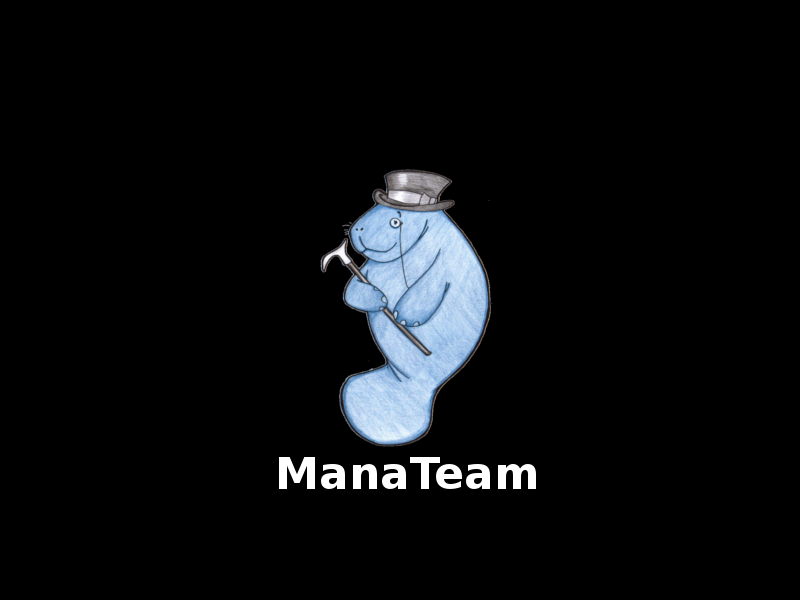
\includegraphics[keepaspectratio=true,scale=0.30]{images/logoMT.png}
\end{figure}
\begin{figure} [!h]
    \centering
    \caption{Tecnologias utilizadas}
    
\includegraphics[keepaspectratio=true,scale=0.30]{images/tecnologias.png}
\end{figure}
\begin{figure}[!h]
    \centering
    \caption{Classificação Indicativa}
    
\includegraphics[keepaspectratio=true,scale=0.30]{images/classificacao_indicativa.png}
\end{figure}

\section{Telas}
\section{Câmera e HUD}

\section{Controles}
O jogador poderá usar como forma de controle para o jogo o teclado do computador ou ainda controles para computadores, mais conhecidos como joysticks. A tabela presente nessa seção apresenta as devidas funcionalidades de ambas as opções dentro do jogo.

\begin{longtable}{|c|c|}
\caption{Controles do jogo}
\\
\hline
\multicolumn{2}{|c|}{Lista de comandos do jogo}
\\
\hline

\includegraphics[scale=0.3]{images/360_Dpad.png}

\includegraphics[scale=0.3]{images/kW.png} 

\includegraphics[scale=0.3]{images/kA.png}

\includegraphics[scale=0.3]{images/kS.png}

\includegraphics[scale=0.3]{images/kD.png}
& Movimentar o personagem na tela
\\
\hline

\includegraphics[scale=0.3]{images/360_RT.png}

\includegraphics[scale=0.3]{images/kShift.png}
 & Correr (na direção selecionada)
\\
\hline

\includegraphics[scale=0.3]{images/360_RB.png}

\includegraphics[scale=0.3]{images/kCtrl.png}
& Rolar (na direção selecionada) 
\\
\hline

\includegraphics[scale=0.3]{images/360_LB.png}

\includegraphics[scale=0.3]{images/kAlt.png}
& Agachar e andar agachado (pressionando algum botão direcional)
\\
\hline

\includegraphics[scale=0.3]{images/360_LT.png}

\includegraphics[scale=0.3]{images/kL.png}
& Ataque com arma secundária
\\
\hline

\includegraphics[scale=0.3]{images/360_A.png}

\includegraphics[scale=0.3]{images/kJ.png}
& Ataque principal (No menu: selecionar opção)
\\
\hline

\includegraphics[scale=0.3]{images/360_B.png}

\includegraphics[scale=0.3]{images/kK.png}
& Pegar item no chão (No menu: negar opção)
\\
\hline

\includegraphics[scale=0.3]{images/360_X.png}

\includegraphics[scale=0.3]{images/kQ.png}
& Usar item 
\\
\hline

\includegraphics[scale=0.3]{images/360_Start.png}

\includegraphics[scale=0.3]{images/kP.png}
& Pausar jogo (acessa o menu de pausa) 
\\
\hline
\end{longtable}
\newpage
\section{A história do jogo}

   Início da 2a Guerra Mundial. A Alemanha invadiu a Polônia, levando a França e o Reino Unido a declarar guerra à Alemanha. O personagem, Edmond Gauthier - um sargento do exército francês - é um homem com um forte senso de honra que lidera bravamente seu exército frente ao inimigo alemão.
   
Em uma missão de resgate na Polônia, Edmond Gauthier e seu exército sofrem uma emboscada, planejada com o principal objetivo de impedi-los de resgatar os reféns judeus que seriam levados ao campo de concentração alemão ainda em construção. Embora a emboscada tenha causado algumas baixas, Edmond consegue alcançar os reféns, porém tarde demais. Ao se aproximar do local, ele percebe que os reféns já haviam sido executados e estavam sendo removidos do caminhão que continha a câmara de gás, uns dos últimos remanescentes da 1ª Guerra Mundial.
   
    Mesmo tendo falhado na missão, o exército francês ataca os alemães, numa espécie de revanche e  aprisiona-os. O superior de Edmond define então que os soldados nazistas aprisionados devem ser fuzilados, o que abala Edmond. Embora seja claro que os nazistas são um mal crescente, o código de honra de Edmond não o permite assassinar homens indefesos, sem a menor chance de revidarem ou sequer se protegerem. No entanto, como a ordem veio de um superior, Edmond é obrigado a obedecer e fuzila os nazistas aprisionados. Após essa missão mal sucedida, e com a crescente ameaça alemã, Edmond resolve voltar ao seu lar na França para se despedir de sua família e os mandarem para a Inglaterra, onde supostamente estariam mais protegidos.
    
    Em 1940, a Alemanha contorna a Linha Magnot - barreira de defesa que cobria toda a fronteira entre a França e a Alemanha, criada pela França após a 1a Guerra Mundial para evitar ataques surpresa e garantir mais tempo de resposta aos franceses em caso de um ataque frontal – vindo pelas densas florestas de Ardenas, único local desprotegido, pois acharam que os tanques alemães não conseguiriam atravessar a floresta. O General Weygand, recentemente nomeado, tomou ações imediatas para conter os alemães. Edmond então é enviado juntamente com o exército francês para conter os alemães. Durante a missão, Pierre Dante (NOME PROVISÓRIO), amigo de Edmond fica sob a mira do fogo inimigo. Edmond, logo parte em sua defesa, abatendo um soldado inimigo de pequeno porte. Ao investigar o corpo do inimigo, Edmond percebe que o soldado era uma criança, de aparentemente menos que 15 anos, o que o deixa perturbado. 
    
    Dois dias depois, ainda tentando conter os alemães, seu esconderijo é atacado por um tanque, desmoronando sobre suas cabeças. Edmond percebe então que Pierre ficou preso nos escombros. Ao tentar resgatar o amigo, acaba notando que o mesmo já se encontrava praticamente sem pulso e desacordado. Edmond decide então, mesmo contra sua vontade, abandonar o amigo e os demais soterrados e foi ao encalço dos alemães.
    
    O exército francês recua enquanto aguarda reforços e, ao receber informes da situação da Europa, descobre que a cidade inglesa onde sua família encontrava-se refugiada foi fortemente bombardeada pelos exércitos alemães. Esse era então o fim para Edmond Gauthier. Nada mais que ele amava lhe restava, além de amargas lembranças dos últimos e turbulentos meses. No entanto, uma missão mais precisava ser cumprida: parar os alemães.
    
    Os alemães, por outro lado, estavam muito fortalecidos e, mesmo com todo o empenho do exército francês e inglês, eles conseguiram avançar adentro do território francês. Edmond e mais alguns oficiais são então aprisionados e torturados em longos interrogatórios. Após obter as informações que necessitavam, os alemães aprisionaram os oficiais no campo de concentração de Bergen- Belsen (ou apenas Belsen) para utilizá-los depois como moeda de troca por oficiais alemães.
    
    Edmond não suporta a pressão causada pelas massivas perdas em sua vida e começa a agir de forma estranha, sendo constantemente atormentado pelas lembranças de seus entes queridos. Sendo considerado como louco, começa a receber uma série de medicações fortes que o deixa 'dopado' por meses a fio. A droga, que ainda estava em experimentação,  é tão forte que começa a afetar as lembranças de Edmond, que lentamente começa a se esquecer de todas as perdas bem como de quem ele próprio é, vivendo em um estágio próximo ao do vegetativo, apenas obedecendo ordens.
    
    Um dia, durante a manutenção do sistema de segurança do campo de concentração, uma pane ocorre no sistema elétrico e a segurança do complexo é comprometida. Praticamente todas as celas do complexo se destravam, o que causa uma tentativa de fuga em massa. Os guardas locais fazem o possível para conter os detentos, enquanto tentam comunicar-se com os campos próximos para solicitar reforços. Edmond, ainda meio sob o efeito dos medicamentos, tenta fugir também, sem atrair a atenção dos guardas. 
    
    Edmond precisará agora utilizar tudo que ainda se lembra para poder sobreviver. Isso significa se esconder nas sombras e atrás de objetos para evitar ser visto pelos guardas. Ou então, quando fugir do guarda não for opção, Edmond precisará eliminá-lo para prosseguir. O complexo em que ele se encontra possui 7 alas divididas em 3 andares, e para fugir ele precisará encontrar chaves específicas que dão acesso aos demais andares/alas até que ele alcance o salão central, que dá acesso aos jardins que por sua vez levam à uma densa floresta, possibilitando uma fuga mais “segura”.
    
    Além de lidar com os guardas, Edmond precisará enfrentar outros seres, fantasmas que habitam sua mente. Esses fantasmas possuem características específicas que o relembram fatos importantes de sua vida. Esses fantasmas são, na verdade, suas lembranças de todas as mortes que o impactaram de alguma forma. No entanto, ele precisará lidar com essas lembranças e não só recordá-las como também aceitá-las para conseguir fugir do inferno em que se encontra. Caso contrário, ele será completamente consumido pela insanidade cada vez mais próxima dele, nesse ambiente completamente hostil e cheio de armadilhas, aguardando-o em cada sala. 

\section{Personagem Principal}

\section{Principais Personagens do Mundo do Jogo}
O personagem principal do jogo é o Edmond Gauthier, no entanto, alguns outro personagens também compõe o universo do jogo, apresentados como inimigos do personagem. Essa seção apresenta esses personagens e um pouco de sua relação com o personagem.

\subsection{Fantasma dos soldados fuzilados}
Como previamente descrito na história do jogo, Edmond não consegue lidar com algumas mortes, como no caso de alguns soldados que, embora inimigos, não morreram de forma digna, segundo o pensamento do Edmond. 
	
	A forma do personagem tem o objetivo de lembrar o Edmond sobre o significado daquele personagem. Isso justifica os furos que o mesmo tem no corpo, representando os tiros disparados nos soldados fuzilados. [INSERIR AQUI IMAGEM E DESCRIÇÃO DO FANTASMA IN GAME E VERSÀO CUTSCENE]
	
	Esse fantasma aparece para o Edmond na primeira fase para impedi-lo de alcançar o andar inferior.

\subsection{Fantasma do soldado criança}
 O fantasma referente ao soldado criança se parece um pouco com o fantasma dos soldados fuzilados pois esse também era um soldado inimigo. Edmond também é perturbado pelo fato de ter matado a sangue frio uma criança, mesmo que o tenha feito para garantir a segurança de seu amigo e aliado de guerra. [INSERIR AQUI IMAGEM E DESCRIÇÃO DO FANTASMA IN GAME E VERSÀO CUTSCENE]
 
 Esse fantasma irá aparecer na segunda fase do jogo. Por representar o fantasma de uma criança, esse fantasma irá tentar pregar "peças" no jogador, como rindo em momentos aleatórios da fase, e  aparecendo em momentos diferentes do primeiro fantasma.
 
\subsection{Fantasma dos reféns da câmara de gás}
Esse fantasma, que tem a base do seu corpo formada por gás, representa uma das maiores falhas de Edmond durante a guerra, a falha na missão de resgate dos reféns judeus na Polônia, como já relatado na história do jogo. [INSERIR AQUI IMAGEM E DESCRIÇÃO DO FANTASMA IN GAME E VERSÀO CUTSCENE]

A pressão causada por essa lembrança na mente de Edmond é tão forte ou até maior que as outras e isso impacta diretamente na relação dele com o fantasma e com a fase em si. O fantasma estará presente em mais momentos da fase, interagindo direta e indiretamente com o Edmond com maior frequência que os anteriores. Esse fantasma estará na terceira fase do jogo.

\subsection{Fantasma do amigo de Edmond}


\subsection{Fantasma da esposa de Edmond}

\subsection{}

\section{NPCs}
\section{Mecânicas Universais}
\section{Inimigos}
\subsection{Policiais}
\subsubsection{Policial fácil}
\subsubsection{Policial médio}
\subsubsection{Policial difícil}
\subsection{Loucos}
\subsection{Fantasmas}
Os fantasmas são, na verdade,personagens que só existem dentro da cabeça do Edmond. A função deles é fazer com que Edmond consiga aceitar os fardos adquiridos ao longo da guerra e supere as perdas.

\section{Sistema de Pontuação}
\section{Saúde}
\section{Power-Ups}
\section{Economia}
\section{Níveis}

\section{O início do jogo}
    O jogo se inicia no último andar do campo de concentração de Belsen. Edmond nota que a cela e tenta fugir. O personagem estará em sua cela no início do jogo. O objetivo de cada fase é procurar a chave que dá acesso á fase seguinte. Essa chave está em algum local aleatório das fases que são geradas de forma aleatória. Seu formato pode mudar de uma fase para outra, mas será sempre um objeto que destrava uma porta específica em alguma sala para a fase seguinte. Toda vez que o jogador perder (for pego por um guarda) o mapa é carregado novamente. Na história, a justificativa para essa mecânica é que a cada vez que ele é capturado e consegue fugir novamente, ele pensa em como ele conseguiria fugir se a estrutura fosse diferente.
  
    Na primeira fase o primeiro inimigo a aparecer será o segurança nível fácil, que fica parado, girando ao redor do próprio eixo, em busca de detentos. Se o guarda avistar o jogador, o jogador terá um tempo para reagir até que o guarda convoque reforços. Inicialmente esse tempo de ação está estimado em 3 a 5 segundos para que o jogador saia da sala que se econtra ou elimine o guarda. Esse guarda eliminado torna-se um fantasma que ficará vagando pelas salas, dificultando progresso do personagem.
  
    Ao encontrar a chave, que estará em alguma sala aleatória, o jogador terá que procurar (caso ainda não tenha achado) a porta que abre com aquela chave. No entanto, ao conseguir a chave, um fantasma especial, exclusivo de cada fase, aparecerá e irá perseguir o jogador, que deve fugir do fantasma até encontrar a porta que dá acesso á próxima fase. Feito isso o jogador terá concluído a fase 1. O processo se repete para as demais fases. No entanto, inimigos, itens e objetos diferentes surgirão à medida que o personagem progrida no jogo

\section{Progresso do Jogo}
\section{Objetos Colecionáveis}
\section{Músicas e Efeitos Sonoros}
\end{document}
